
\section{Objetivo}
Que el alumno pueda comparar los resultados de las operaciones de su clase \classname{Factor} usando la aplicación \classname{SamIam} \par

\section{Desarrollo e implementaci\'on}

\noindent La práctica consiste en extender su clase \classname{Factor} para que pueda recibir consultas y contestarlas adecuadamente, las consultas serían de la forma:

\begin{itemize}
  \item \(P(<Var_i>, \dots <Var_j>)\)
  \item \(P(<Var_i>=0, <Var_k>=1, \dots <Var_j>)\)
  \item \(P(<Var_i> | <Var_k>=1, \dots <Var_j>)\)
\end{itemize}

\noindent Por Ejemplo:

\begin{itemize}
  \item \(P(A,B,C)\)
  \item \(P(A=0,B=2,C)\)
  \item \(P(A|B=2,C)\)
  \item \(P(A=1|B=2,C=0)\)
\end{itemize}


\subsection{Usando SamIam}

\noindent Deberán crear una nueva red del tipo \classname{in-out degree}, como lo muestra la siguiente figura:

\begin{figure}[H]
  \centering
  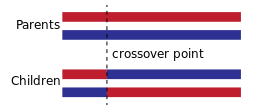
\includegraphics[scale=0.5]{practica6/screen1.png}
  \caption{}
\end{figure}

\noindent Después pueden crear nuevos nodos usando el botón que contiene un círculo de color amarillo como ícono:

\begin{figure}[H]
  \centering
  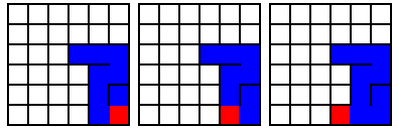
\includegraphics[scale=0.5]{practica6/screen5.png}
  \caption{}
\end{figure}

\noindent Al momento de darle doble click al nodo, les aparecerá la siguiente ventana:

\begin{figure}[H]
  \centering
  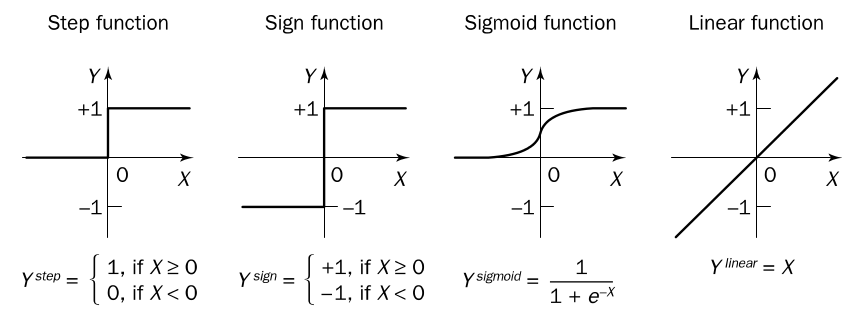
\includegraphics[scale=0.5]{practica6/screen3.png}
  \caption{}
\end{figure}

\noindent Donde pueden agregar estados de la variable y asignarle una probabilidad a cada estado.\\

\noindent Para entrar al modo de consulta deberán dar click al botón que tiene como ícono dos flechas circulares, como se muestra en la figura:

\begin{figure}[H]
  \centering
  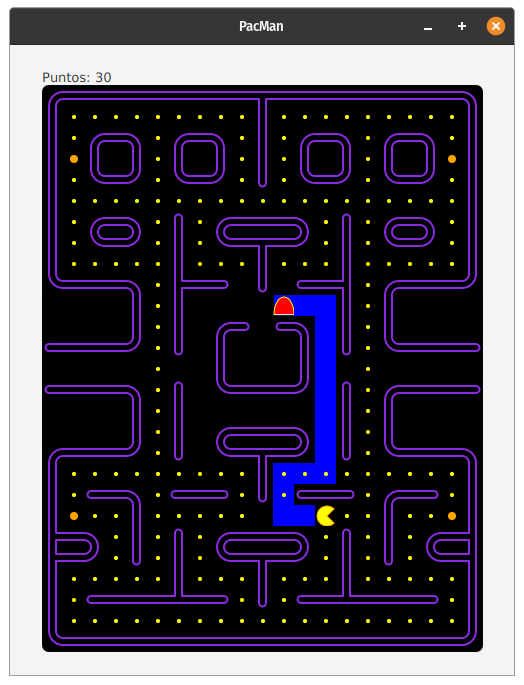
\includegraphics[scale=0.5]{practica6/screen6.png}
  \caption{}
\end{figure}

\noindent Al final, les deberá quedar algo como:

\begin{figure}[H]
  \centering
  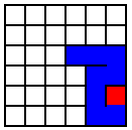
\includegraphics[scale=0.4]{practica6/screen4.png}
  \caption{}
\end{figure}

\subsection{Implementaci\'on}

\noindent Deberán cargar en su aplicación el problema de la complicada de pedro, y deberán hacer las siguientes consultas:

\begin{enumerate}
  \item \(P(li \mid \neg mp, \neg fin)\)
  \item \(P(JP)\)
  \item \(P(ma, ap, vp)\)
  \item \(P(mp, ap, jp, bp, vp \mid \neg lf, fin, \neg it, \neg e)\)
\end{enumerate}


\noindent También deberán usar \classname{SamIam}, cargar el mismo problema y comparar si los resultados obtenidos por su aplicación concuerdan con lo que arroja \classname{SamIam}.\\\par

\noindent Recuerden que la probabilidad conjunta está dada por la suma de los eventos atómicos en los cuales las variables pregunta tienen los valores asignados. Es posible calcular esta probabilidad multiplicando todos los factores de la red bayesiana y marginalizando las variables que no sean variables preguntas.\\\par

\noindent Recuerden también la fórmula:\\ \[ P( A \mid B ) = {P(A,B) \over P(B)} \]


\section{Requisitos y resultados}

\noindent Se deberá entregar un reporte con las observaciones y resultados del punto anterior.\\\par


